\documentclass[12pt]{article}  
%%Read the manual for other options. 

\pagestyle{empty} %%Eliminates page numbers
%%\input rmb_macros
%%Collect your favorite macros in a 
%%separate file

%\input amssym.def
%\input amssym
%\input mssymb
%%Defines additional symbols



\usepackage{graphics}
\usepackage{amsmath,amssymb,amsthm, multicol,tikz,pgf,subfig,enumerate}
\usetikzlibrary{arrows.meta}
%\usepackage[pdftex]{graphicx}
\usepackage{epsf}
\newenvironment{theorem}
{\begin{proof}[Theorem]}
{\end{proof}}
%%Use to include pictures. 

%\newcommand{\comment}[1]{}
%\newcommand{\sobolev}[2]{W^{#1,#2}}
%\newcommand{\sobolev}[2]{L^#2_#1}
%%Some examples of macros or new commands.

%\addtolength{\oddsidemargin}{-.75in}
%\addtolength{\evensidemargin}{-.75in}
%\addtolength{\textwidth}{1.5in}
%\addtolength{\topmargin}{-1in}
%\addtolength{\textheight}{2.25in}
%%Set margins, defaults are ok. 

\begin{document}
% \begin{center}
% {\bf \Large Some Games}
% \vspace{0.2cm}
% \hrule
% \end{center}
\section*{A Counting Game}
This game involves two players. The first player chooses a positive integer less than or equal to 10. Then the second player adds a positive integer less than or equal to 10 to this first number. This goes back and forth, where the winner is whoever chooses a number so that the grand total is 101. Play a few rounds of this game.

\subsection*{Questions}
\begin{enumerate}
	\item Does either player have a winning strategy? What does it look like?
	\vspace{4cm}
	\item What if we adjust the numbers? Say the winning number is 77 and players take turns adding positive integers no greater than 8. What if the winning number is $N$ and players add positive integers no greater than $m$?
	\vspace{4cm}
	\item What if instead, whichever player is the first to bring the total to a number greater than or equal to 101 \textit{loses}? What's the strategy now?
\end{enumerate}

\newpage

\section*{Chomp}
\begin{figure}[h]
	\centering
    \subfloat{{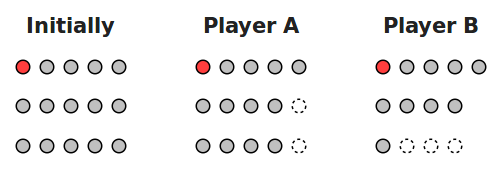
\includegraphics[scale=.5]{chomp1} }}%
    \\
    \subfloat{{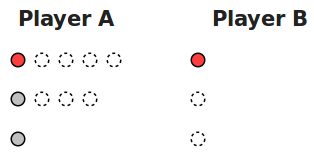
\includegraphics[scale=.5]{chomp2} }}%
    \caption{Chomp}
    %\label{fig:example}%
\end{figure}
Chomp is played with two players and a 5 by 3 grid of Skittles. Players take turns selecting a Skittle. Upon selection, the player eats that Skittle and any Skittle below and to the right of it. The player who eats the Skittle in the top left-hand corner loses.\\

\noindent Chomp away!

\subsection*{Questions}
\begin{enumerate}
	\item Does either player appear to have any advantage over the other?
	\vspace{1.5cm}
	\item Experiment with differently sized grids. Do your strategies change?
	\vspace{1.5cm}
	\item Suppose the second player has a winning strategy (that is, they can win regardless of what the first player does). Explain what the first player can do to show that this is actually impossible.
\end{enumerate}

\newpage

\section*{A Tic-Tac-Toe-Like Game}
\begin{figure}[h]
	\centering
    \subfloat[Empty Board]{{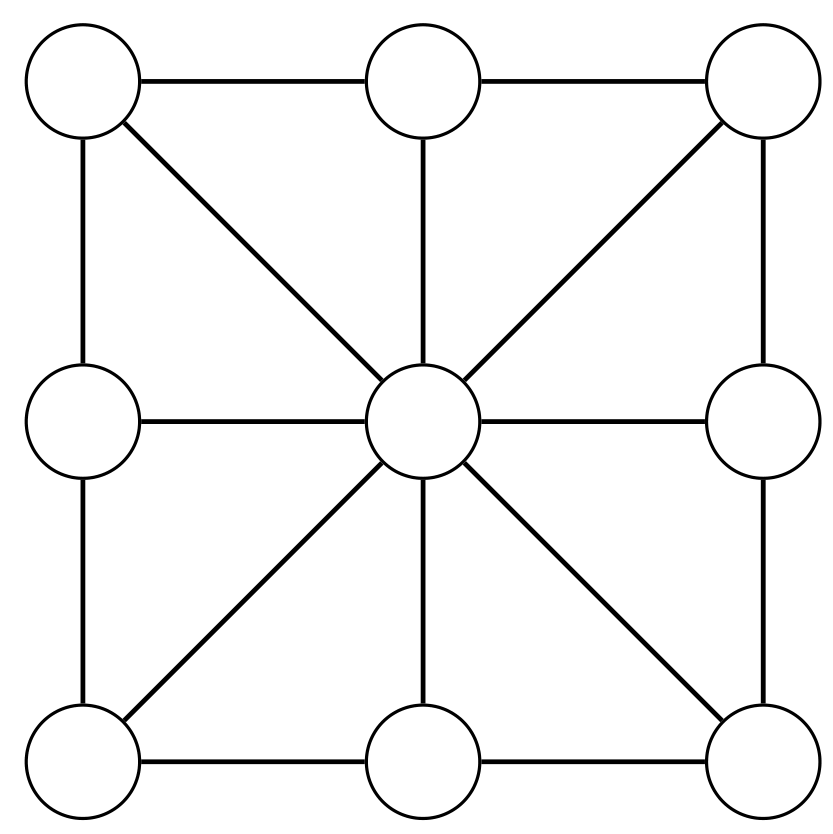
\includegraphics[scale=.2]{achi_empty} }}%
    \qquad
    \subfloat[Full Board]{{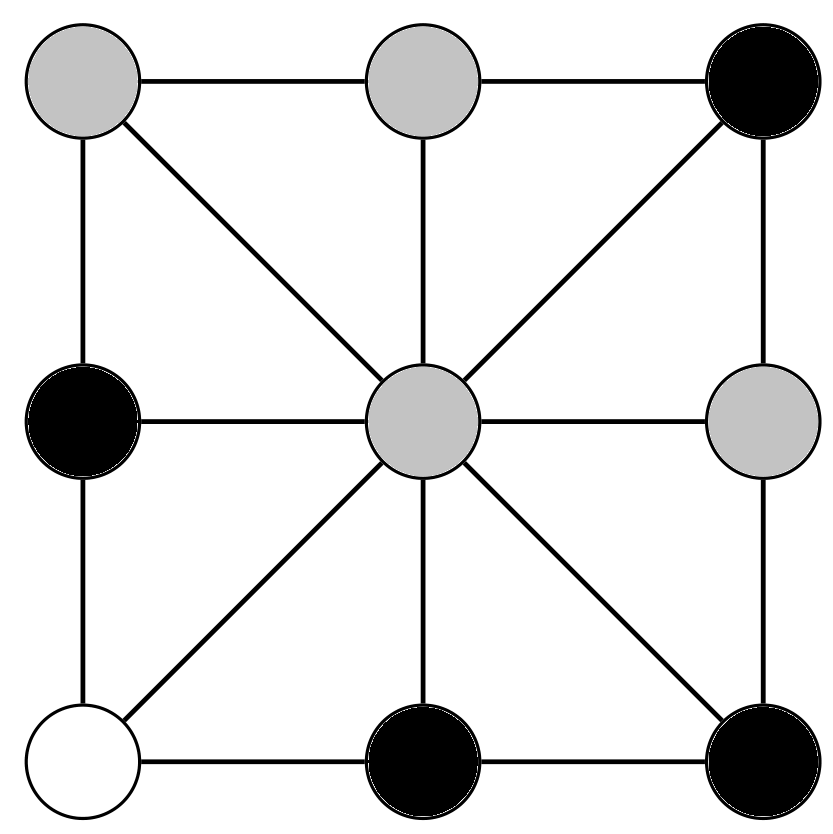
\includegraphics[scale=.2]{achi_full} }}%
    \\
    \subfloat[Gray's Next Move]{{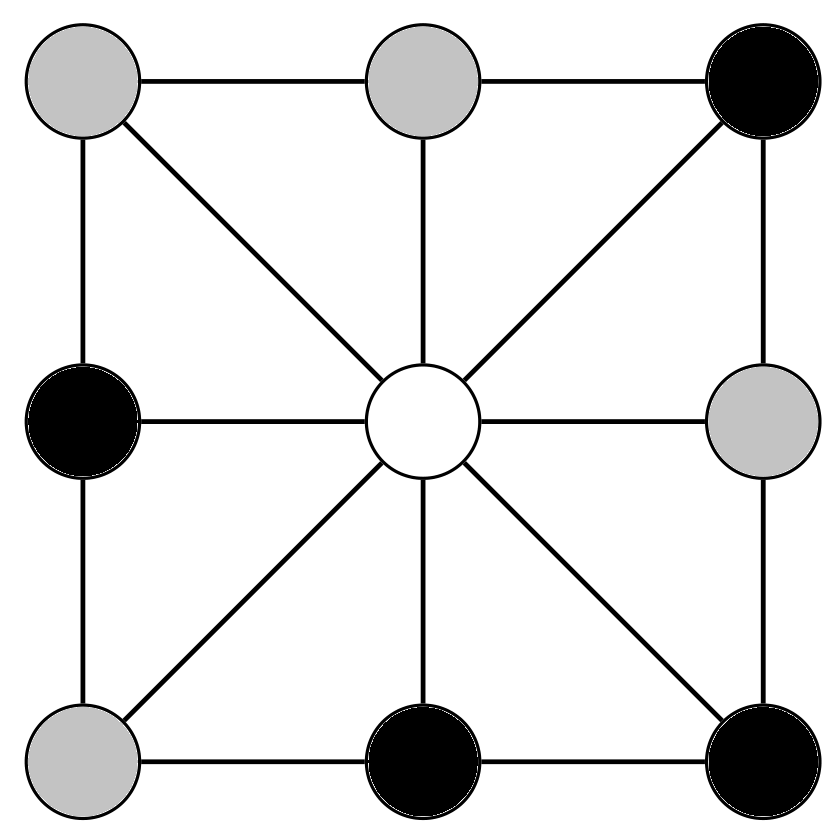
\includegraphics[scale=.2]{achi_next.png}}}
    \caption{}
    %\label{fig:example}%
\end{figure}
\noindent Two players start with four counters each. One player has gray counters, the other black. Just like in tic-tac-toe, this game is played on a three by three grid and players take turns placing their counters on the grid, trying to be the first to get three in a row.\\

\noindent Once both players have run out of counters, the players take turns sliding their already placed counters along the board's edges into the only empty space. Say the gray player goes first. The players go back and forth until they reach the sate shown in Figure 1(b). Neither player has three in a row yet, so play continues. Gray's only valid move is to slide their center counter the the lower-left space. Now black can move any of their counters to the center space. This continues until a player ends up with three counters in a row.\\

\noindent Play a few rounds of this game.

\subsection*{Questions}
\begin{enumerate}
	\item Is this game guaranteed to end?
	\vspace{4cm}
	\item Are any spaces on the board more valuable than others? Why or why not?
	\vspace{4cm}
	\item Does either player have an advantage? If so, can they be guaranteed to win with perfect play, regardless of what their opponent does?
\end{enumerate}

\newpage 



\section*{Hex}
\begin{figure}[h]
	\centering
    \subfloat[Empty Board]{{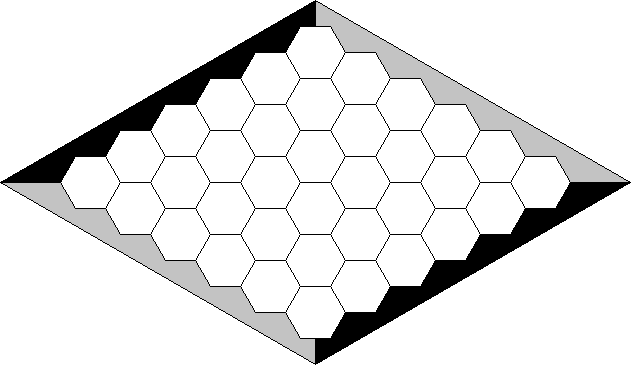
\includegraphics[scale=.3]{hex_empty} }}%
    \qquad
    \subfloat[A Few Moves In]{{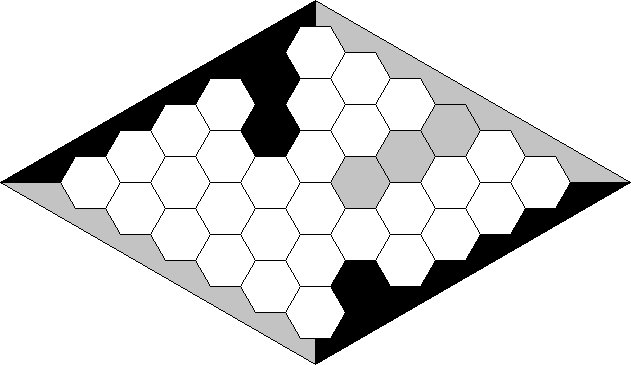
\includegraphics[scale=.3]{hex_progress} }}%
    \\
    \subfloat[Gray Wins!]{{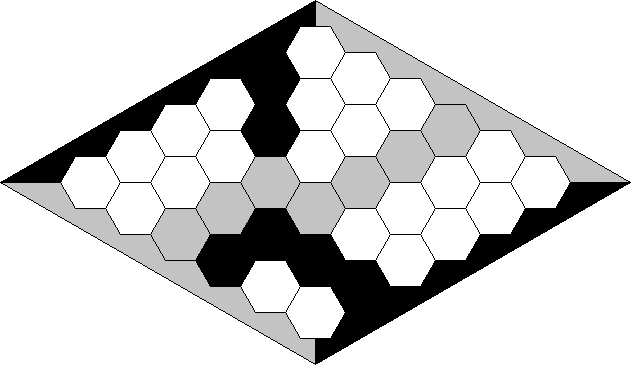
\includegraphics[scale=.3]{hex_end}}}
    \caption{}
    %\label{fig:example}%
\end{figure}
\noindent Hex is played with two players on a hexagonal grid. Each player has their own color, say gray or black. Players take turns coloring in hexagons with their assigned colors. Each player's goal is to build a connected path of their own color joining opposite sides of the board marked by their color. The first player to connect their sides wins. The four corners belong to both players.\\

\noindent Play some hex!


\subsection*{Questions}
\begin{enumerate}
	\item Let's show that Hex never ends in a draw.
	\begin{enumerate}[(a)]
		\item Say the game ends with a full board. Starting with a hexagon vertex at a corner, imagine drawing a path along the edges between hexagons of different colors. Can this path intersect itself (forming a loop)?
		\vspace{3cm}
		\item Why can't this path terminate in the middle of the board or on either side of the board (not counting corners)?
		\vspace{3cm}
		\item Why can't this path connect opposite corners?
		\vspace{3cm}
		\item Conclude that one player must have won.
		\vspace{3cm}
		\item Can you think of an easier (but maybe less rigorous) way of proving this?
		\vspace{3cm}
	\end{enumerate}

	\item Now that you know that somebody must win, can either player come up with a winning strategy?
\end{enumerate}

\newpage
\begin{figure}[h]
	\centering
	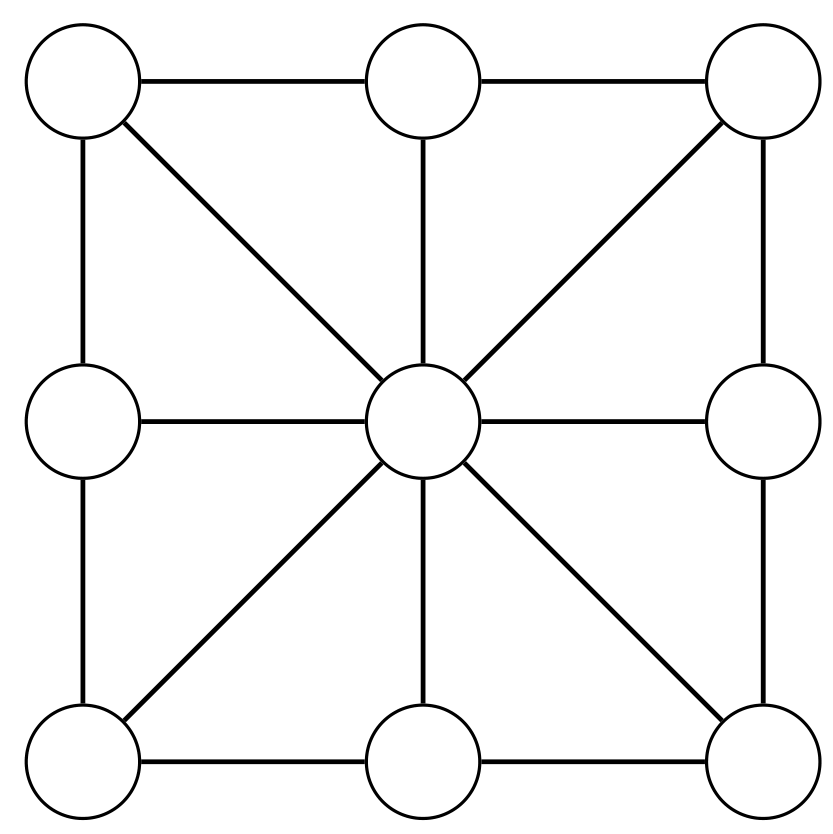
\includegraphics[scale=.7]{achi_empty.PNG}
\end{figure}

\newpage

    Begin with a Hex board completely filled with hexagons marked with either X or O (indicating which player played on that hexagon).\\
    Starting at a hexagon vertex at the corner of the board where the X side and O sides meet, draw a path along the edges between hexagons with different X/O markings.\\
    Since every vertex of the path is surrounded by three hexagons, the path cannot self-intersect or loop, since the intersecting portion of the path would have to approach between two hexagons of the same marking. So, the path must terminate.\\
    The path cannot terminate in the middle of the board since every edge of the path ends in a node surrounded by three hexagons--two of which have to be differently marked by construction. The third hexagon must be differently marked from the two adjacent to the path, so the path can continue to one side or the other of the third hexagon.\\
    Similarly, if the sides of the board are considered to be a solid wall of X or O hexagons, depending on which player is trying to connect there, then the path cannot terminate on the sides.\\
    Thus the path can only terminate on another corner.\\
    The hexagons on either side of the line form an unbroken chain of X hexagons on one side and O hexagons on the other by construction.\\
    The path cannot terminate on the opposite corner because the X and O markings would be reversed at that corner, violating the construction rule of the path.\\
    Since the path connects adjacent corners, the side of the board between the two corners (say, an X side) is cut off from the rest of the board by an unbroken chain of the opposite markings (O in this case). That unbroken chain necessarily connects the other two sides adjacent to the corners.\\
    Thus, the completely filled Hex board must have a winner.

 \newpage

    Either the first or second player must win, therefore there must be a winning strategy for either the first or second player.\\
    Let us assume that the second player has a winning strategy.\\
    The first player can now adopt the following defense. He makes an arbitrary move. Thereafter he plays the winning second player strategy assumed above. If in playing this strategy, he is required to play on the cell where an arbitrary move was made, he makes another arbitrary move. In this way he plays the winning strategy with one extra piece always on the board.\\
    This extra piece cannot interfere with the first player's imitation of the winning strategy, for an extra piece is always an asset and never a handicap. Therefore the first player can win.\\
    Because we have now contradicted our assumption that there is a winning strategy for the second player, we are forced to drop this assumption.\\
    Consequently, there must be a winning strategy for the first player.\\



% \newpage
% \begin{tikzpicture}
% \begin{scope}[every node/.style={circle,thick,draw}, minimum size=1cm]
%     \node (v1) at (0,0) {};
%     \node (v2) at (0,3) {};
%     \node (v3) at (0,6) {};
%     \node (v4) at (3,0) {};
%     \node (v5) at (3,3) {};
%     \node (v6) at (3,6) {};
%     \node (v7) at (6,0) {};
%     \node (v8) at (6,3) {};
%     \node (v9) at (6,6) {};   
% \end{scope}

% \begin{scope}[every node/.style={fill=white,circle},
%               every edge/.style={draw=black,very thick}]
%     \path (v1) edge (v2);
%     \path (v2) edge (v3);
%     \path (v1) edge (v4);
%     \path (v3) edge (v6);
%     \path (v1) edge (v5);
%     \path (v4) edge (v5);
%     \path (v5) edge (v6);
%     \path (v3) edge (v5);  
%     \path (v2) edge (v5);  
%     \path (v4) edge (v7);  
%     \path (v5) edge (v8);  
%     \path (v5) edge (v7);  
%     \path (v5) edge (v9);  
%     \path (v6) edge (v9);  
%     \path (v7) edge (v8);  
%     \path (v8) edge (v9);  
% \end{scope}
% \end{tikzpicture}


\end{document}